%!TEX encoding = UTF-8 Unicode
% !TeX spellcheck = en_GB

%%%%%%%%%%%%%%%%%%%%%%%%%%%%%%%%%%%%%%
\chapter{ Overview of Higgs pair production at colliders }\label{chap:overviewDiHiggs}
%%%%%%%%%%%%%%%%%%%%%%%%%%%%%%%%%%%%%%
\par The determination of the shape of the Higgs potential is an essential part of the LHC physics programme. Unlike other Higgs measurements reviewed in this thesis, the light Yukawa and Higgs-self couplings are exceptionally hard to probe.  This is evident from the conclusion of ~\autoref{chap:4topSingleHiggs} for the case of trilinear Higgs coupling. We have seen that the effectiveness of using single-Higgs signals to probe the Higgs trilinear coupling is challenged by other weakly constrained operators also affecting these signals. Thus, Higgs pair production remains the only direct way to access this elusive interaction. 
\par The production of Higgs in pairs has roughly~$ 10^{-3} $ of the signal producing single Higgs at the LHC. Higgs pair production, with Higgs, decays considered, has a cross-section of~$ \sim 1 \si{\femtobarn}$, in the SM. Sensitivity to the SM Higgs pair production will hence only be reached in the high luminosity phase of the LHC~\cite{Cepeda:2019klc}. The quartic coupling, that requires NLO corrections to Higgs pair or can be directly accessed in triple Higgs production, both of which remain elusive at the LHC~\cite{Plehn:2005nk}. The main advantages for Higgs pair production in determining the Higgs trilinear self-coupling come from the dependence of the cross-section on $\lambda_3$ at the LO level, as well as the fact that the rest of SMEFT operators entering this process~(see eq~\eqref{HH-smeft}) can also be constrained from other processes. This will improve the constraints on these operators when both Higgs pair and other Higgs measurements are combined cf.~\cite{DiVita:2017eyz}\footnote{The same could not be said for non-linear HEFT operators; such operators require Higgs pair production to be directly probed.}. However, the inclusion of light quark Yukawa couplings modifiers, e.g.~$ C_{u\phi}$ and $C_{d \phi}$ can influence potential bounds on $C_\phi$. 
\par This chapter starts by reviewing the theoretical status of the dominant process for Higgs pair production, beginning with the gluon fusion in~\autoref{ggFhh}. Then, the other subdominant channels will be briefly reviewed in~\autoref{otherhh}.  Afterwards, I overview the experimental efforts in probing these rare yet fascinating processes in~\autoref{exphh}. Finally, I present  in~\autoref{summtrilinear} a summary of the potential for Higgs pair production in probing Higgs elusive interactions.
%%%%%%%%%%%%%%%%%%%%%%%%%%%%%%%%%%
\section{Higgs pair production by gluon fusion \label{ggFhh}  }
%%%%%%%%%%%%%%%%%%%%%%%%%%%%%%%%%%
\par The dominant process for Higgs pair production at the LHC~(and hadron colliders in general) is the gluon fusion channel via top quarks in the loops, while the beauty-quark loops contribute less than~$1\%$.
%
\begin{figure}[!htpb]
	\centering
	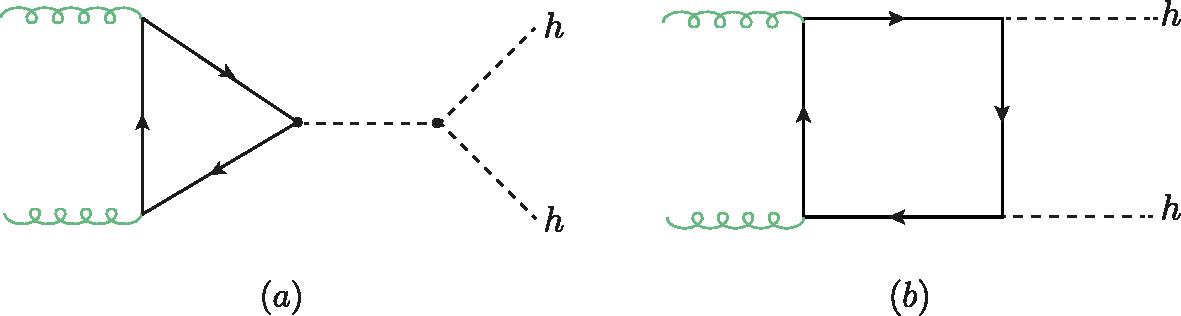
\includegraphics[width = 0.8\textwidth]{./figures/di-higgs-LO-SM}
	\caption{Feynman diagrams for the ggF process of Higgs pair production in the SM.} 
	\label{fig_ggf_sm}
\end{figure}
%
This process is well-studied at leading order~(LO) analytically~\cite{EBOLI1987269, GLOVER1988282, DICUS1988457, Plehn:1996wb}.  The higher-order computations are significantly more complicated to perform compared to the gluon fusion production of single-Higgs. As has been outlined in~\autoref{chap:hz} for $gg \to Zh$, the computation of multi-scale amplitudes at two-loop order is extremely challenging and requires numerical approaches or approximations. The first attempt to compute the NLO corrections to di-Higgs were via the HTL approximation~\cite{Dawson:1998py, Altenkamp:2012sx,Grigo:2014jma}, improved by reweighing with the full LO matrix element squared. These corrections are implemented in~\texttt{HPAIR}~\cite{Plehn:1996wb}. These corrections are large, with a K-factor of $ \sim 2$.  This prompted more calculations with inclusion of top quark mass effects~\cite{deFlorian:2013uza,Maltoni:2014eza,Grigo:2015dia,Degrassi:2016vss}, which improved the stability of the HTL expansion as well as corrected the cross-section by $\sim 10\%$. 
\par Later, the threshold resummation effects of the HTL have been included in \cite{Shao:2013bz}. This approach, however, is not sufficient to produce corrections to the differential cross-section, as the HTL fails for $M_{hh}^2/4m_t^2 \lesssim 1$. The cross-section though peaks at $ M_{hh}\approx 400$ GeV, hence this approximation only describes well a small part of the phase space. Using the numerical evaluation of the two-loop integrals, it is possible to obtain exact results with full top quark mass dependence, see refs.~\cite{Borowka:2016ypz,Borowka:2016ehy,Baglio:2018lrj}. Nonetheless, this comes at the cost of computational power required to evaluate the cross-section. Fast and flexible implementations at NLO QCD can be obtained from analytical computations, i.e. small $\pt$~\cite{Bonciani:2018omm}, high energy~(HE) expansion~\cite{Davies:2018ood} and expansions in small Higgs mass~\cite{Xu:2018eos,Wang:2020nnr}. The latter covers of the whole $M_{hh}$ spectrum. The NNLO cross-section has been computed numerically in~\cite{Grazzini:2018bsd}, and also at differential level~\cite{deFlorian:2016uhr}. analytical NNLO computations are only available in the HTL~\cite{deFlorian:2013jea}. Also, NLO+ NNL analytical results have been obtained by~\cite{deFlorian:2015moa}. Parton shower matching for NLO Higgs pair production has been computed  in~\cite{Jones:2017giv}, which was essential for the \texttt{POWHEG} implementation for di-Higgs, with NLO corrections computed from a grid that has been made available by ~\cite{Heinrich:2017kxx,Heinrich:2019bkc,Heinrich:2020ckp}. 
\par  The small $\pt$ and HE expansions can be bridged using Pad\'e  approximants~\cite{Bellafronte:2022jmo}.  The matching between the results across low and high energy intervals of $m_{hh}$ shows the strength of the Pad\'e  approximants technique. The LO Higgs pair production with SMEFT operators is available in \texttt{SMEFTatNLO} model~\cite{Degrande:2020evl} for \Madgraph. Calculation of higher-order corrections to Higgs pair production in EFT have been performed in refs.~\cite{Grober:2014zva,Grober:2015cwa,deFlorian:2017qfk,Buchalla:2018yce}.
\par In the analysis shown in the next chapter, the Higgs pair production cross-section at NNLO QCD order was used in accordance with according to the LHC Higgs working group recommendations~\cite{Dittmaier:2012vm,deFlorian:2016spz}:
\begin{equation}
	K = \frac{\sigma_{NNLO}}{\sigma_{LO}}, \;\;\;\;\; K_{14 \mathrm{TeV}} \approx 1.71.
\end{equation}
The $^3$LO corrections in the HTL have been performed in ref.~\cite{Chen:2019fhs}.
\subsection{Theoretical uncertainties}
There are four dominant sources of the theoretical uncertainties for Higgs pair production:
\begin{enumerate}
	\item Scale uncertainty: coming form the arbitrariness of scale choice. This is used as a measure of missing higher-order corrections.
	\item PDF uncertainties: as a result of the uncertainty in the PDF fitting and modelling.
	\item $\alpha_s$ running uncertainty: originating from the initial value (i.e. $\alpha_s(M_Z) $).
	\item The choice of the quark mass renormalisation scheme that involves $m_t$ appearing in the loop propagators and in the top Yukawa.
\end{enumerate}
\par The computation of the PDF and $\alpha_s$ uncertainties is described in~\cite{Martin:2009bu, Demartin:2010er}.
In order to calculate the scale uncertainties, the cross-section was computed with different $ \mu_R$ and $\mu_F$ values ranging between:
\begin{equation}
	\frac{M_{hh}}{4} \leq \mu_R/\mu_F  \leq \,M_{hh}
\end{equation}
\par The combination of the $m_t$ renormalisation and scale uncertainties can be found in \cite{Baglio:2020wgt}.
The total 14 TeV ggF $hh$, cross-section at different orders in computation with its uncertainties is shown in~\autoref{ggf_xsres}, which indicates that the uncertainties are dominated by the $m_t$ renormalisation scheme of $\sim -18\%$ uncertainty in the lower envelope.  This is a significant part of the uncertainty budget and needs to be resolved by including N$^3$LO corrections to ggF $hh$. Such corrections are available hitherto only in the HTL~\cite{Chen:2019lzz,Chen:2019fhs}; however, in this approximation, the $m_t$ uncertainty cannot be computed.
%
\begin{table}
	\centering
	\begin{tabular}{ccccc}
		\toprule
		& $ \sigma$	[fb] & Scale [fb] & PDF$+\alpha_s$ [fb]& Total [fb] \\
		\midrule
		SM    (LO)  &  $ 21.45$    &   $ \,^{+4.29}_{-3.43}$   & $\pm 1.46$   &  $ \,^{+4.53}_{-3.73}$ \\
		SM   (NLO)~\cite{Baglio:2012np}  &  $ 33.89$   &   $ \,^{+6.17}_{-4.98}$   & $ \,^{+2.37}_{-2.01}$   &  $ \,^{+6.61}_{-5.37}$ \\
		SM   (NNLO)~\cite{Grazzini:2018bsd}  &  $36.69$    &    $ \,^{+0.77}_{-1.83}$   & $\pm 1.10$   &  $ \,^{+1.66}_{-6.43}$ {\tiny(incl. $m_t$ uncertainty~\cite{Baglio:2020wgt})} \\
		\bottomrule
	\end{tabular}
	\caption{Gluon fusion Higgs pair production cross-section at 14 TeV with theoretical  uncertainties, the HTL is computed using HEFT, top running mass, LO, NLO and NNLO QCD corrections. The NLO and NNLO results are taken from the references cited in the table. The LO results are computed via a FORTRAN code. Using the NNPDF30 PDFs~\cite{Ball:2017nwa}, a central scale of $ M_{hh}/$ and $ \alpha_s(m_z) = 0.118$.}
	\label{ggf_xsres}
\end{table}

\section{Other processes\label{otherhh}  }
\par Like single-Higgs production at hadron colliders, the production of Higgs pairs has the same subdominant channels VBF, di-Higgsstrahlung $ Vhh$ and associates production of Higgs pair with top quarks $t\bar hh /t j hh$. Their cross-sections and uncertainties at 14 TeV are shown in~\autoref{table:di-higgs}, while in~\autoref{dihiggs-all} their cross-sections as a function of the centre-of-mass energy $\sqrt{s}$ is shown~\cite{DiMicco:2019ngk}. 
\begin{table}[htbp!]
	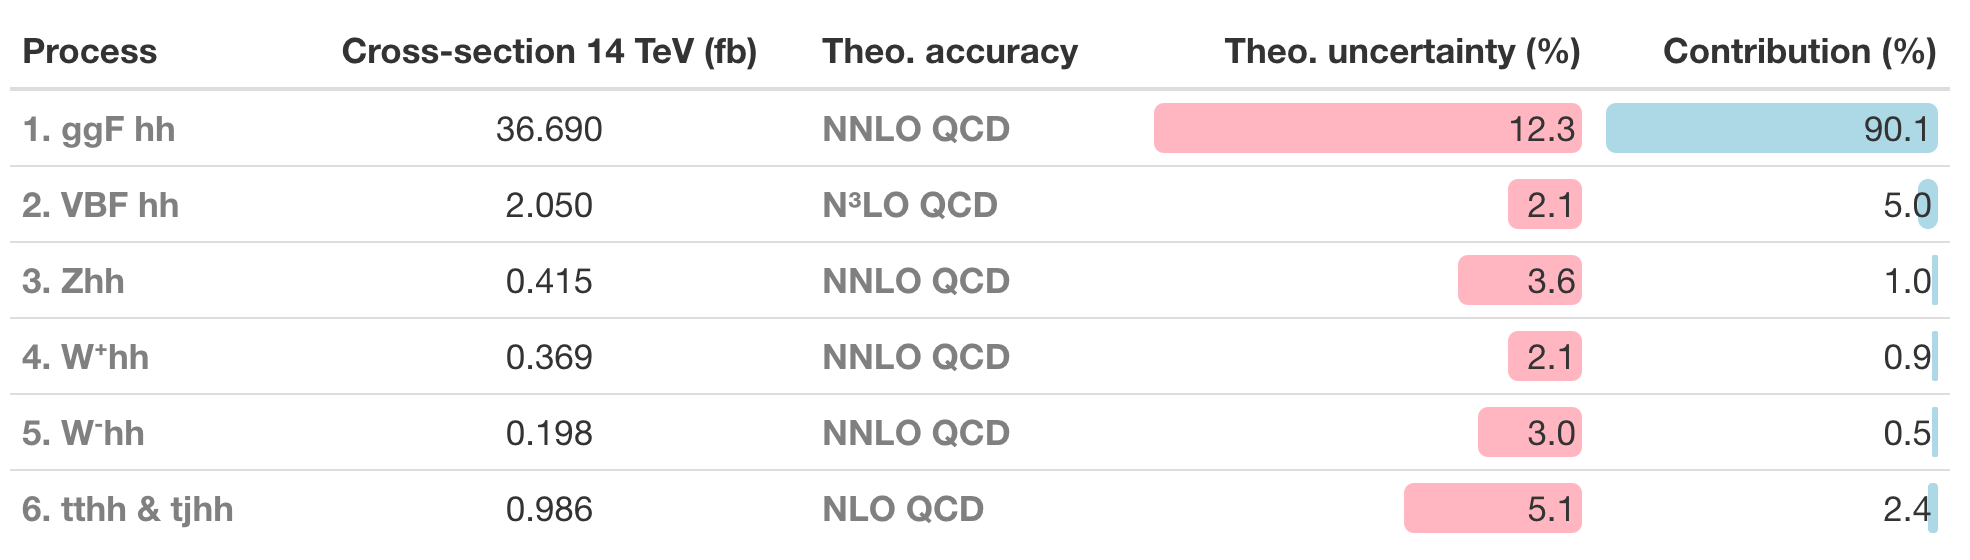
\includegraphics[width=1\textwidth]{hh-table}
	\caption{ Summary of the Higgs pair production processes at 14 TeV LHC. Event generation software implementation of the gluon fusion channel is only available at NNLO theoretical accuracy, despite that N$^3$LO corrections have been performed in~\cite{Chen:2019fhs} \label{table:di-higgs} }
\end{table}
\subsection{VBF $hh$}
\par Vector boson fusion $hh$ production has the second largest cross-section after ggF $hh$, which is calculated up to N$^3$LO~\cite{Baglio:2012np,Ling:2014sne,Dreyer:2018qbw} inclusively and differentially at NNLO~\cite{Dreyer:2018rfu}. The dominant diagrams are analogous to the single Higgs VBF involving the $W/Z$ bosons exchanged in the $t-$channel. The process has the same topology as the off shell single Higgs VBF, with the off-shell Higgs giving two final states ones via the trilinear self-coupling. 
\subsection{Di-Higgsstrahlung}
\par The associated production of the Higgs pair with $W$ and $Z$ bosons has a small cross-section compared to ggF and VBF. This process is known up to NNLO QCD accuracy, including the gluon-fusion component in the full computation~\cite{Baglio:2012np,Li:2016nrr, Li:2017lbf}. 
\subsection{Associated Higgs pair production with $t$-quarks}
\par Sometimes called the di-Higgs bremsstrahlung off top quarks~\cite{DiMicco:2019ngk}, this channel has a steeper dependence on $\sqrt{s}$ than the single Higgs bremsstrahlung $t\bar t h$. One can see, for example, from~\autoref{dihiggs-all} that its cross-section becomes at roughly the same values as the VBF's at large $\sqrt{s}$. Only NLO computations for these channels have been carried out~\cite{Frederix:2014hta}.  All three channels have a relatively small NLO correction compared to ggF, which ranges from 10-30\%. 
\begin{figure}[!htpb]
	\centering
	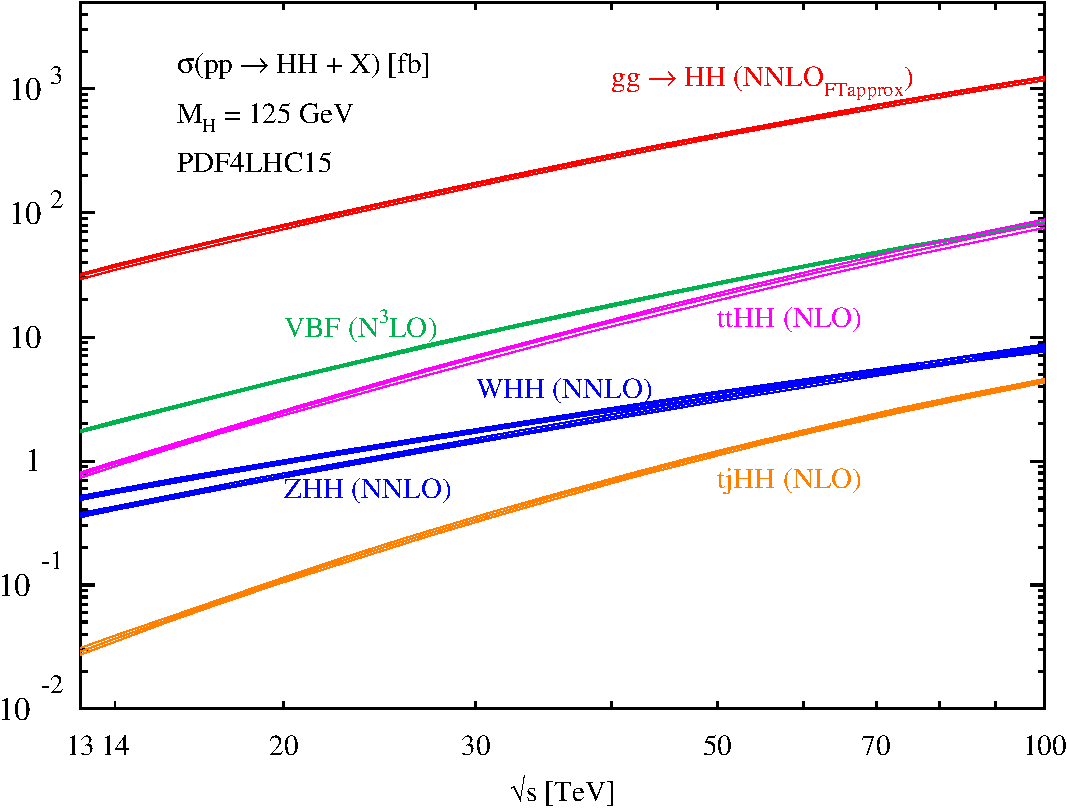
\includegraphics[width = 0.8\textwidth]{./figures/cxn_HH}
	\caption{The cross-section of all Higgs pair production processes at the highest available perturbation order as a function of centre-of-mass energy $\sqrt{s}$.The bands show the uncertainties without the top quark mass renormalisation scheme. This plot is taken from~\cite{DiMicco:2019ngk}.} 
	\label{dihiggs-all}
\end{figure}
%
%%%%%%%%

\section{Experimental overview for Higgs pair production \label{exphh}  }
\par The search for Higgs pair production can be divided into two categories, resonant and non-resonant production. The first searches for heavy resonances that decay into a Higgs pair, while the latter is concerned about the SM scenario or if the NP has a scale beyond the reach of the LHC, i.e. when the EFT limit is valid. In this review, I shall focus on the non-resonant searches, as these are the ones relevant to the focus of this thesis; for a detailed overview of the resonant searches, cf.~\cite{DiMicco:2019ngk}.
%
%\autoref{dihigs-exp} shows the current experimental scopes for detecting non-resonant Higgs pair production by both ATLAS and CMS. The searches are summarised according to the final state:
%\begin{figure}[!htpb]
%	\centering
%	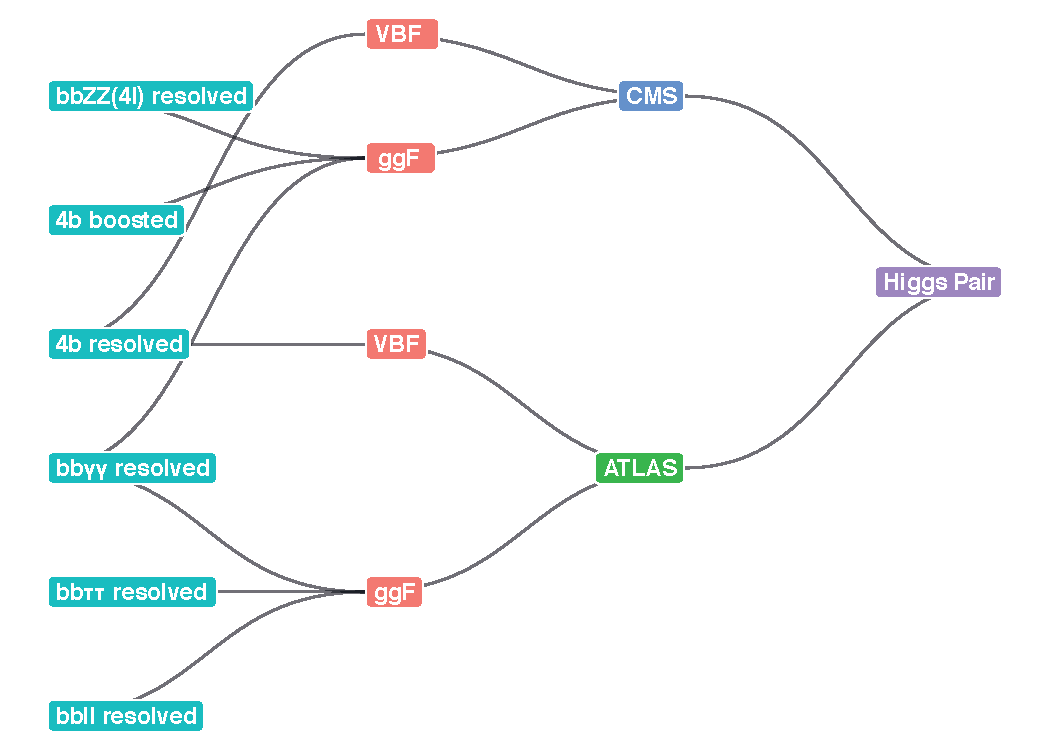
\includegraphics[width = 0.8\textwidth]{./figures/HH-exp-network}
%	\caption{The non-resonant Higgs pair searches conducted by ATLAS and CMS using the full Run-II data.} 
%	\label{dihigs-exp}
%\end{figure}
\subsection*{$hh \to b\bar b b \bar b $}
\par The final state $ hh \to b\bar b b \bar b$ has the highest SM cross-section possible for the Higgs pair but is difficult to probe due to the large QCD background of four b-tagged jets in the final state. CMS~\cite{CMS-PAS-HIG-20-005} has used boosted decision trees~(BDT) for studying this final state for ggF and VBF channels. This allowed for sensitivity on the trilinear and $hhVV$ couplings. Their analysis led to 95\% CL bounds on $\kappa_\lambda \in [-2.3;9.4]$ and $\kappa_{2V} \in [-0.1; 2.2]$.  They have also performed a boosted analysis for the VBF channel by defining two large jets with a jet radius of $\Delta R =0.8$. Despite their analysis not being sensitive to the trilinear self-coupling, it could probe both $\kappa_V$ and  $\kappa_{2V} $, which leads to the most stringent bound on the latter coupling modifier so far  $\kappa_{2V}  \in [0.6;1.4]$. The $\kappa_{2V}=0$ hypothesis is excluded with $ p<0.001$~\cite{CMS-PAS-B2G-21-001}. On the other hand, ATLAS has performed only a resolved analysis for this final state and the VBF production channel~\cite{ATLAS:2020jgy}. Hence they were able to report bounds on $hhVV$ coupling $\kappa_{2V} \in [-0.43;2.56]$. 
\subsection*{$hh \to b\bar b VV $}
\par ATLAS has considered the gluon fusion final state~$hh \to b\bar b \ell \ell$, with the leptons coming from $WW/ZZ$ decays~\cite{ATLAS:2019vwv}. This state covers around $90\%$ of the total~$hh \to b\bar b VV $ signal. Their analysis was divided into two categories: same-flavour and different-flavour leptons. The observed signal strength was lower than the expected one. Hence, no bounds on the self-coupling could be extracted from this search. CMS has carried out a similar analysis but with a requirement to observe four leptons instead of two. That is, they have searched for the final state $hh \to b\bar b( ZZ^*\to 4\ell)$. The 95\% CL upper limit on the signal strength was 30 times the SM one, with bounds on Higgs self-coupling of $\kappa_\lambda \in [-9;14]$~\cite{CMS-PAS-HIG-20-004}. 
\subsection*{$hh \to b\bar b \tau \tau $}
\par This channel has backgrounds coming from real $\tau$'s, such as $t\bar t$ and $Z j$ with heavy jets. In addition to fake $\tau$'s coming from QCD multijet process. A neural network~(NN) has been used by ATLAS~\cite{ATLAS-CONF-2021-052} investigating this channel, using resolved $b$ jets. The extracted bounds on the trilinear self-coupling are $\kappa_\lambda \in [-2.4;9.2]$. 
\subsection*{$hh \to b\bar b \gamma \gamma $}
\par This final state is the most promising for Higgs pair searches. Despite having a lower cross-section than the previous final states with BR of  0.27\% in the SM, it has the highest selection efficiency.  This is due to the low backgrounds and the ability to reconstruct the photons fully. The dominant non-reducible background is QCD/QED production of $b\bar b \gamma \gamma$, which has a cross-section of ~$\sim13\si{\femtobarn}$ at the 14 TeV LHC, more details about the backgrounds of this final states are shown in~\autoref{tab:xsec14}. 
\begin{table}[h!]
	\centering
	\begin{tabular}{cccc}
		\specialrule{.8pt}{0pt}{0pt}
		Channel	        &LO $\sigma$ [fb]	&NLO $K$-fact	&6$\inab$ [\#evt @ NLO]   \\ %& 2$b$-jets[\%]  \\ 
		\specialrule{.8pt}{0pt}{0pt}
		$b\bar b h, y_b^2$	        &0.0648	            &1.5	    &583                \\%&7.7\%  \\
		$b\bar b h, y_by_t$        &-0.00829	        &1.9        &-95                \\%&4.0\%	\\
		$b\bar b h, y_t^2$	        &0.123	            &2.5	    &1,840              \\%&12\%	\\
		$Zh$	        &0.0827	            &1.3	    &645                \\%&21\%   \\
		$\sum\bbh$	    &0.262	            &-	        &2,970              \\%&-      \\
		$\bbaa$	        &12.9	            &1.5	    &116,000            \\%&14\%	\\
		$t\bar th$	    &1.156	            &1.2	    &6,938              \\%&42\%	\\
		%$hh_{\rm SM}$	&0.567	\la{0.053}            &1.72	    &3,492  \la{316}              \\%&32\%	\\ 
		\specialrule{.8pt}{0pt}{2pt}
	\end{tabular}
	\caption{ SM cross-section for the main background processes at 14\ TeV with 6$\iab$ data at the HL-LHC. For $\bbh$ production, the Higgs boson is decayed to a pair of photons. The total production of Higgs associated with $b\bar{b}$ is denoted by $\sum\bbh$ and is the sum of the top four channels.
	}
	\label{tab:xsec14}
\end{table}
\par Both ATLAS and CMS have published searches of this channel using  BDT and NN analyses~\cite{ATLAS:2021jki,CMS:2020tkr}. Though the ATLAS collaboration has reported the strongest 95\% CL bound on $\kappa_\lambda$ thus far, and their result was used in the comparisons in~\autoref{fig:summcphihl-lhc}. In comparison, CMS has reported bounds on both $\kappa_\lambda$ and $\kappa_{2V}$ of $\kappa_{\lambda} \in [-3.3;8.5]$ and $\kappa_{2V} \in [-1.3; 3.5]$.                                                                                       
%\subsection{Prospects for the HL-LHC}
%One of the main goals of the HL-LHC programme is the detection of Higgs pair production. The Higgs pair signal can be observed at $\sim  4- 4.5\sigma $ level~\cite{DiMicco:2019ngk}. The use of machine learning techniques in the analysis of $hh$ searches will be a key factor in the success of these searches~\cite{Cepeda:2019klc}. In~\autoref{sec:mlanalysisly}, the interpretable machine learning technology will be exploited in improving the sensitivity for $hh$ signals at the HL-LHC. With the main focus on the $\bbaa$ final state. As this channel has the highest potential for discovery of di-Higgs production~\cite{Azatov:2015oxa, Baur:2003gp, Baglio:2012np, Kling:2016lay, Barger:2013jfa, Adhikary:2017jtu, Alves:2017ued}. The projected constraints on $\kappa_\lambda$ at the HL-LHC for combined ATLAS and CMS are~$\kappa_{\lambda} \in [0.1,2.3]$~\cite{DiMicco:2019ngk,Cepeda:2019klc}

\section{Summary \label{summtrilinear}  }
\par The Higgs pair production is a missing critical measurement of the SM; it is essential to determine the Higgs potential by directly constraining the Higgs trilinear self-coupling. Moreover, this channel is sensitive to non-linear couplings of the Higgs. Due to the small cross-section of this channel, current searches obtain relatively weak bounds on $\kappa_{\lambda}$ that are comparable with the perturbative unitarity bounds~\cite{DiLuzio:2017tfn}. Nonetheless, the HL-LHC is expected to result in an observation or even discovery of this process, particularly with the help of advanced machine learning techniques.
\par  The observation of Higgs pair production is expected to provide a direct measurement of one of the two ``difficult'' couplings in the SM Higgs sector,  the trilinear Higgs self-coupling. However, as we shall explore in the upcoming chapter, it could also provide a window for observing the Higgs coupling to light quarks, the second challenging coupling class we discussed earlier.
